\documentclass[11pt,twoside,a4paper]{book}
\usepackage[utf8]{inputenc}
\usepackage[czech]{babel}
\usepackage{caption}
\usepackage{subcaption}
\usepackage{minted}
\usepackage{mathtools}
\usepackage{listings}
\usepackage{graphicx}
\usepackage{hyperref}https://www.sharelatex.com/project/5a11a6c3e7e3011e1a88d93e
\usepackage[dvipsnames,hyperref]{xcolor}
\usepackage{pdfpages}
\usepackage{caption}
\usepackage{csquotes}
\usepackage[style=numeric,citestyle=ieee,hyperref,natbib,backend=biber]{biblatex}
\addbibresource{reference.bib}

\definecolor{aliceblue}{RGB}{240,248,255}
\definecolor{wonderland}{RGB}{15,123,196}
\hypersetup{%
    colorlinks=true, linktocpage=true, pdfstartpage=1, 
    pdfstartview=FitV, breaklinks=true, pdfpagemode=UseNone, 
    pageanchor=true, pdfpagemode=UseOutlines,%
    plainpages=false, bookmarksnumbered,
    bookmarksopen=true,%
    bookmarksopenlevel=1,%
    hypertexnames=true, pdfhighlight=/O,%
    urlcolor=wonderland,
    linkcolor=RoyalBlue, 
    citecolor=wonderland,%
    %hyperfootnotes=false,
    %pdfpagelabels,
    pdfsubject={},%
    pdfkeywords={},%
    pdfcreator={pdfLaTeX},%
    pdfproducer={LaTeX}%
}

\let\tmp\oddsidemargin
\let\oddsidemargin\evensidemargin
\let\evensidemargin\tmp
\reversemarginpar

\usepackage{titlesec}
\usepackage{xcolor}
\usepackage{fancyhdr}
\usepackage{graphicx}
\usepackage{titling}

\definecolor{darkaccent}{HTML}{007AC2}
\definecolor{lightaccent}{HTML}{107AC2}

%page style
\pagestyle{fancy}
\renewcommand{\headrulewidth}{0pt}
\renewcommand{\footrulewidth}{0pt}

%section
\titleformat{\section}
[hang]
{\Large\bfseries}
{
\color{darkaccent}
\raisebox{-2pt}{
    \rule{0.35cm}{1em}
}
\color{black}
\sffamily
\thesection
}
{10pt}
{
\color{lightaccent}
\sffamily
\Large\bfseries
}
 
%subsection
\titleformat{\subsection}
[hang]
{\large\bfseries}
{
\color{darkaccent}
\raisebox{-2pt}{
    \rule{0.35cm}{1em}
}
\color{black}
\sffamily
\thesubsection
}
{10pt}
{
\color{lightaccent}
\sffamily
\large\bfseries
}

%subsubsection
\titleformat{\subsubsection}
[hang]
{\normalsize\bfseries}
{
    \empty
}
{10pt}
{
\color{darkaccent}
\raisebox{-2pt}{
    \rule{0.35cm}{1em}
}
\color{black}
\sffamily
\thesubsubsection
\color{lightaccent}
\hspace{1em}
\normalsize\bfseries
}
 
%chapter
\titleformat
{\chapter} 
[display] 
{\bfseries\huge} 
{
    \color{darkaccent}
    \raisebox{0em}{
        \rule{0.35cm}{1em}
    }
    \color{black}
    \sffamily
    \chaptertitlename \ \Huge\thechapter
} 
{-0.75em}
{
    \color{darkaccent}
    \raisebox{-2pt}{
        \rule{0.35cm}{1.5em}
    }
    \sffamily
    \color{lightaccent}
}

\renewcommand{\maketitle}
{
    \begingroup % Create the command for including the title page in the document
    \hbox
    { % Horizontal box
        \color{darkaccent}
        \rule{0.35cm}{\textheight} % Vertical line
        \color{black}
        \hspace*{0.05\textwidth} % Whitespace between the vertical line and title page text
        \parbox[b]{0.9\textwidth}
        { % Paragraph box which restricts text to less than the width of the page
            
            \noindent\sffamily\large\textbf{\TypeOfWork}\vspace{\baselineskip}\\
            
            \begin{tabular}{lc}
                
\includegraphics[width=3cm]{ctulogo} & 
                
                \color{lightaccent}\sffamily\Large\textbf{
                    \parbox[b]{5cm}{
                        České \\
                        vysoké\\
                        učení technické\\
                        v Praze
                    }
                    \vspace{1em}
                } \\
                \Huge\color{lightaccent}\sffamily\textbf{F3} & 
                \parbox[b]{5cm}{
                    \textbf{\Faculty} \\
                    \textbf{\Department}
                }
            \end{tabular}
            \vspace{3cm}
            
            \color{lightaccent}\sffamily\huge\textbf{\WorkTitle}\\
            
            \Large\color{black}\textbf{\FirstandFamilyName} \\
            \normalsize\textbf{\StudProgram} \\

            \vspace{6.5cm}
            
            \normalsize
            \textbf{\Date}\\
            \labelSupervisor: \Supervisor
        }
    }
    \endgroup
}

\newcommand{\splitpage}[3]{
    \begingroup
    \begin{center}
    \color{lightaccent}\huge\sffamily\centering\textbf{#1}
    \end{center}
    \raisebox{0.83\textheight}{\parbox[t]{0.45\textwidth}{
        #2
    }}
    \color{darkaccent}
    \hspace{1mm}
    \rule{0.35cm}{0.85\textheight} % Vertical line
    \hspace{1mm}
    \color{black}
    \raisebox{0.83\textheight}{\parbox[t]{0.45\textwidth}{
        #3
    }}
    \endgroup
} %Template

\author{Jan Dryk}

\newcommand\Date{\today}
\newcommand\Department{Katedra počítačů}
\newcommand\Faculty{Fakulta elektrotechnická}
\newcommand\University{České vysoké učení technické v Praze}
\newcommand\labelSupervisor{Vedoucí práce}
\newcommand\labelStudProgram{Studijní program}
\newcommand\labelStudBranch{Obor}
\newcommand\TypeOfWork{Bakalářská práce}
\newcommand\StudProgram{Softwarové technologie a management}
\newcommand\StudBranch{Softwarové inženýrství}
\newcommand\WorkTitle{Mobilní klient restauračního systému}
\newcommand\FirstandFamilyName{Jan Dryk}
\newcommand\Supervisor{Ing. Martin Komárek}

\begin{document}
\chapter{Manuál}
\label{ch:manual}
\graphicspath{{appendixes/Manual/}}

\section{Instalační příručka pro vývojáře}

Aby bylo možno přiložený kód znovu zkompilovat a zpustit, je nutné mít nainstalované a licencované nástroje Xamarin.
Ty lze stáhnout ze stránek firmy Xamarin (\url{http://xamarin.com/download}).
Pro kompilaci iOS aplikace je nutné iOS SDK, které je dostupné pouze pro OS X. 
Lze využít Xamarin Studio pro Mac nebo Visual Studio s Xamarin Build Serverem na zařízení s OS X a iOS SDK.
Aplikace byla vyvinuta ve Visual Studiu a projekt nebyl v Xamarin Studiu testován.
Pro spuštění aplikace na přístroji je nutné mít zařízeni registrované s vývojářským účtem pro iOS a s ním i správně nastavený XCode.
Z tohoto důvodu není dodaný instalační balíček pro iOS.

\begin{sloppypar}
Návod pro nastavení přístroje lze nalézt na adrese
\url{http://developer.xamarin.com/guides/ios/getting_started/installation/device_provisioning/}.

Návod pro nastavení vývojového prostředí s Visual Studiem lze nalézt na adrese \url{http://developer.xamarin.com/guides/ios/getting_started/installation/windows/}.
\end{sloppypar}

Pro kompilaci aplikace pro Android je nutné Android SDK. 
Instalaci správného Android SDK zařídí instalační program platformy Xamarin.\\

Spouštění projektu ve Visual Studiu nebo v Xamarin Studiu je velmi podobné. 
Nejdříve vyberte kýžený projekt jako výchozí (Solution Explorer $>$ pravé tlačítko myší na projekt $>$ Set as Startup Project) a dejte Debug v panelu nástrojů.
Pokud je vše korektně nastaveno zobrazí se zvolený emulátor a aplikace se na něm nainstaluje a spustí.
V případě, že chcete aplikaci spustit na zařízení, připojte zařízení k počítači (K build serveru u iOS + Visual Studio) a vyberte jej na panelu nástrojů jako cílové.

\subsection{Testy}

Unit Testy jsou v projektu CashBob.Mobile.UnitTests, který je v podstatě samostatnou aplikací.
Pro spuštění testů nejdříve vyberte tento projekt jako výchozí (Solution Explorer $>$ pravé tlačítko myší na projekt $>$ Set as Startup Project) a dejte Debug v panelu nástrojů.\\

UI Testy jsou jako normální Unit testy spustitelné na počítači pomocí zabudovaného test runneru Visual Studia.
Momentálně jsou nakonfigurované jen pro platformu Android.
Před spouštěním testů je nutné zapnout vyžadovaný emulátor na kterém mají testy běžet.

\section{Uživatelský manuál aplikace}

K instalaci aplikace na zařízení s operačním systémem Android stačí stáhnout .apk soubor na Váš Android přístroj a spustit ho.
Operační systém Vás potom provede instalací.
Aplikace vyžaduje minimální verzi Android v4.4 (KitKat).

K instalaci aplikace na zařízení s operačním systémem iOS je potřeba mít zařízení zaregistrováno u vývojářského účtu pro iOS.
Instalace je pak nejsnažší s kompilací pomocí IDE.

\subsection{Server}

Tento krok je volitelný, jelikož lze využít testovací server v cloudu, který byl připraven jako součást této práce.

Lokální server spustíte pomocí programu "CashBobServer.exe" z přibaleného archivu (CashBobServerShade-distribution.zip). \\

Funčnost serveru lze ověřit zadáním adresy \url{http://localhost:9998/rest} do Vašeho prohlížeče, pokud se Vás prohlížeč dotáže na jmého a heslo, vše je v pořádku.

\subsection{Nastavení a přihlášení}

Nejdříve je nutné nastavit IP adresu serveru.
Tu lze nastavit ze stránky nastavení na kterou se dostanete stisknutím tlačítka Settings (viz obr. \ref{fig:loginpage}).\\

Tablet a počítač s CashBob serverem musí být na stejné síti.
Do políčka IP Adresa vyplňte IP adresu počítače, na kterém běží server.
V případě cloudu je adresa o 52.10.102.132.
Adresu lze zjistit pomocí cmd a příkazu ipconfig. 
Měnu není nutné vyplňovat, ale pro české koruny se vyplňuje "\ Kč".\\

Správnost IP adresy lze otestovat stisknutím tlačítka "Check Connection" viz obr. \ref{fig:settingspage}.
Bez funkčního spojení nebude možno se přihlásit.  

Z nastavení se dostanete tlačítkem zpět nebo stiskem názvu stránky (Settings na obrázku \ref{fig:settingspage}).

K Přístupu do aplikace je nutné se přihlásit pod svým přihlašovacím jménem.
Výchozí jméno a heslo pro přihlášení je "admin" a "pass" u přibaleného i cloudového serveru. 

\begin{figure}[h]
\centering
\begin{minipage}{.5\textwidth}
  \centering
  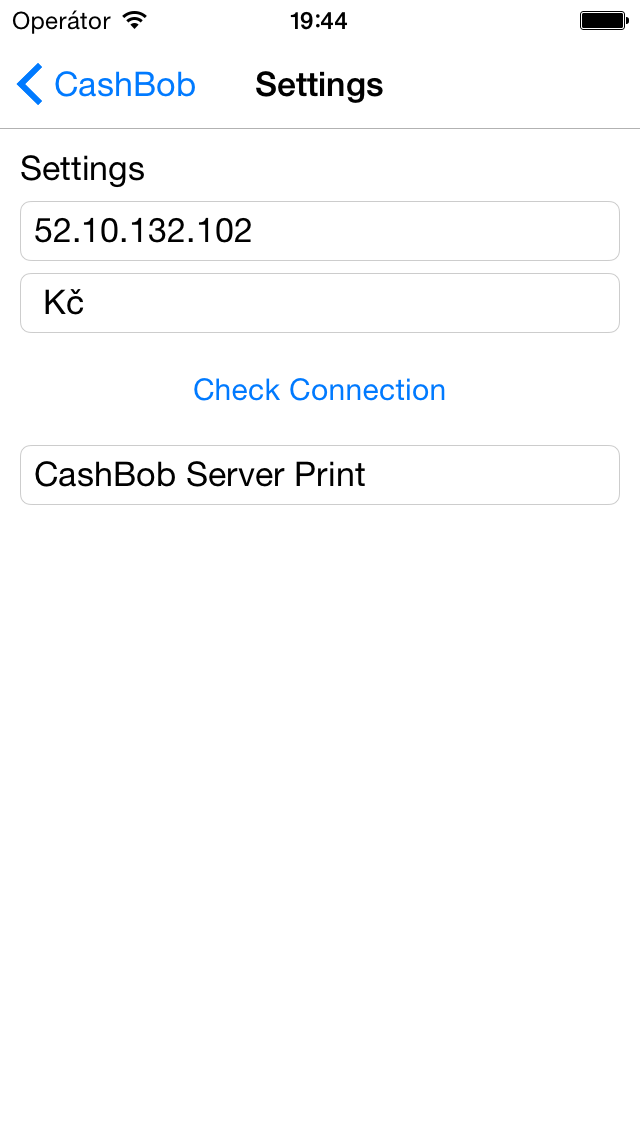
\includegraphics[width=.95\textwidth]{settings.png}
  \captionof{figure}{Nastavení}
  \label{fig:settingspage}
\end{minipage}%
\begin{minipage}{.5\textwidth}
  \centering
  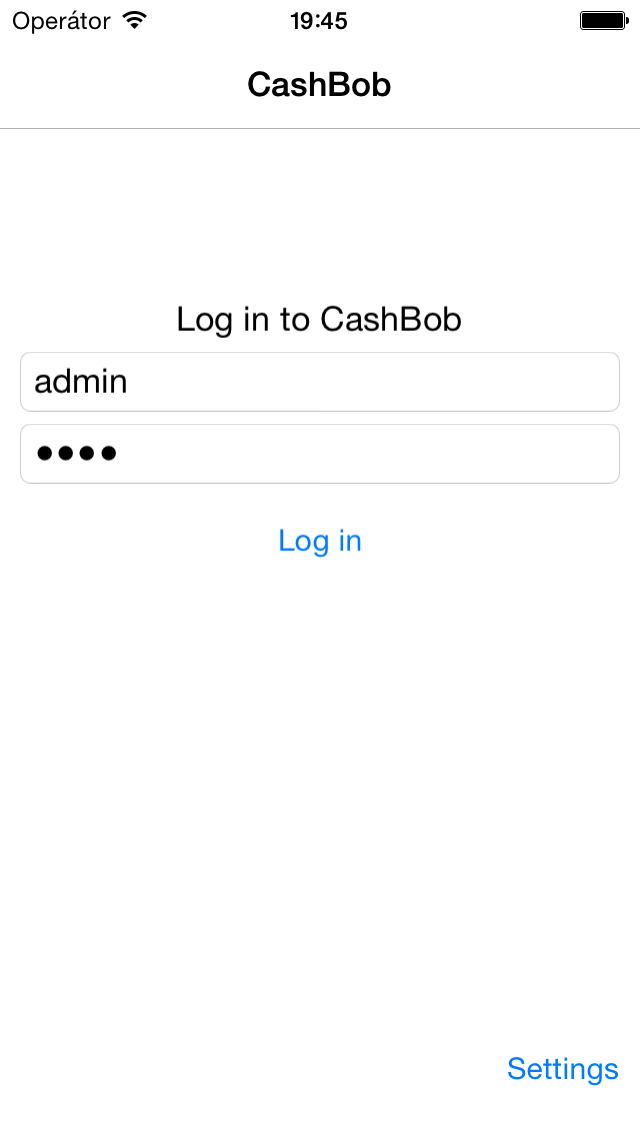
\includegraphics[width=.95\textwidth]{login.png}
  \captionof{figure}{Přihlášení}
  \label{fig:loginpage}
\end{minipage}
\end{figure}

\subsection{Připojení tiskárny Star Micronics SM-T300}
Jak zprovoznit a připojit tiskárnu k zařízení je popsáno v manuálu tiskárny, který je dostupný na \url{http://www.starmicronics.com/support/manual.aspx?printerCode=SM-T300}.
Po nabití baterie stiskněte tlačítko POWER po dobu 5 vteřin pro zapnutí tiskárny.
Potom spárujte tiskárnu se svým zařízením pomocí technologie Bluetooth.
Tiskárna se objeví pod názvem Star Micronics a PIN její 1234.
Po úspěšném spárování můžete s tiskárnou tisknout.

\subsection{Funkce aplikace}

Po přihlášení do aplikace se dostanete na stránku s existujícími účty viz obrázek \ref{fig:accountspage1}.
Jako většina stránek v aplikaci má i tato stránka vysouvací postranní panel.
Tento panel bude na telefonech schovaný a musí být vysunut tahem z levého okraje obrazovky.
Na tabletech bude vyditelný vždy pokud bude na displayi dostatek místa.
Z této stránky lze procházet účty, kterých seznam naleznete v postranním panelu viz obrázek \ref{fig:accountspage1}.
V hlavní části obrazovky je pak přehled aktivních objednávek právě zvoleného účtu jak je vidět na obrázku \ref{fig:accountspage2}.

Z této stránky jsou na horní liště nástrojů dostupné další funkce ve formě ikonek.
Ikonky nemají pod nimy popis z důvodu nedostatku místa, ale popis lze ukázat u jakékoliv ikonky v aplikaci podržením prstu na ikonce.
Jedná se o přesouvání položek mezi účty, vytvoření nového účtu, vytvoření nové objednávky na právě zvolený účet a placení položek zleva do prava. \\

\begin{figure}[h]
\centering
\begin{minipage}{.5\textwidth}
  \centering
  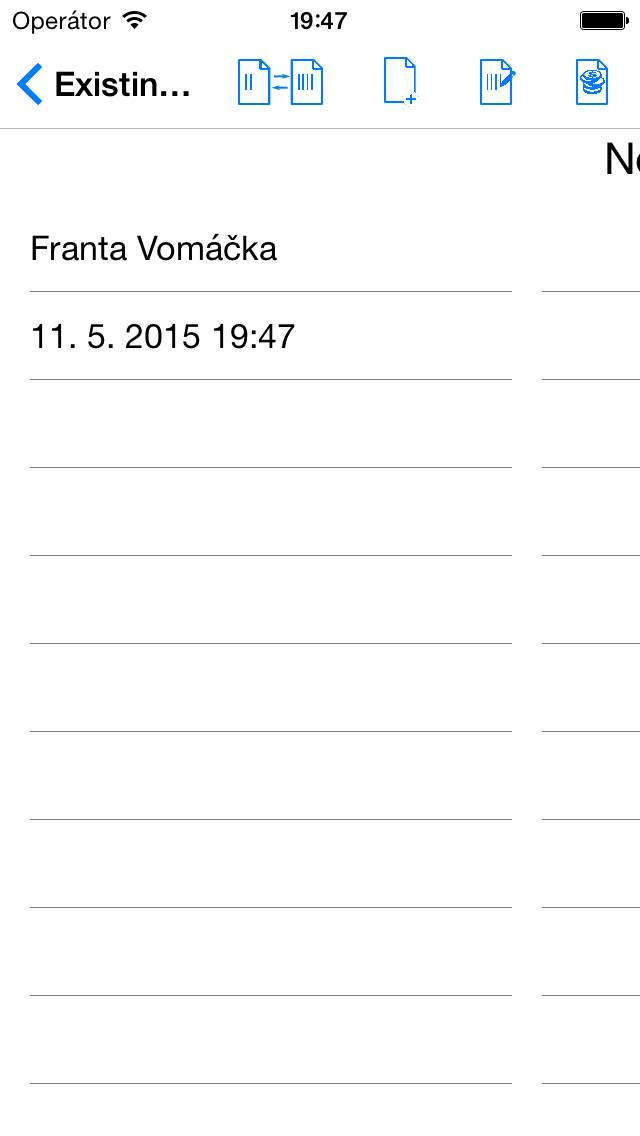
\includegraphics[width=.95\textwidth]{accounts1.png}
  \captionof{figure}{Existující účty}
  \label{fig:accountspage1}
\end{minipage}%
\begin{minipage}{.5\textwidth}
  \centering
  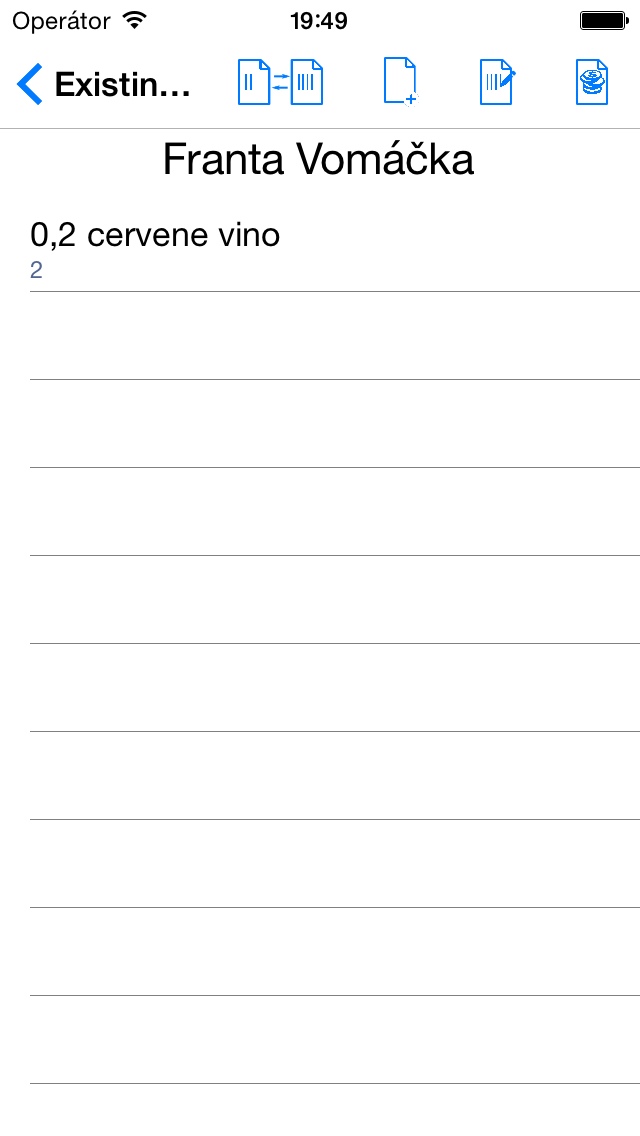
\includegraphics[width=.95\textwidth]{accounts2.png}
  \captionof{figure}{Obsah účtu}
  \label{fig:accountspage2}
\end{minipage}
\end{figure}

První z funkcí je přesun položek mezi účty.
Tato funkce se stává z dvou kroků a umožňuje přesunout aktivní objednávky z jednoho účtu na druhý.
V prvním kroku jak ukazuje obrázek \ref{fig:moveorderspage1} vybereme zdrojový a cílový účet.
Pokud cílový účet ještě neexistuje, můžeme ho vytvořit zvolením na liště nástrojů ikonky vytvořit nový účet (první ikona zleva).
Až vybereme cílový a zdrojový účet potvrdíme volbu pomocí ikonky potvrdit (druhá zleva).

V druhém kroku vybíráme které položky přesunout.
Položky volíme k přesunu pomocí tlačítka plus u dané položky.
Počet zvolených položek jednoho typu lze upravit pomocí příslušného tlačítka mínus.
V liště nástrojů jsou dostupné dvě funkce.
První z nich (zleva) potvrdí výběr, druhá automaticky přesune všechny dostupné položky.\\

\begin{figure}[h]
\centering
\begin{minipage}{.5\textwidth}
  \centering
  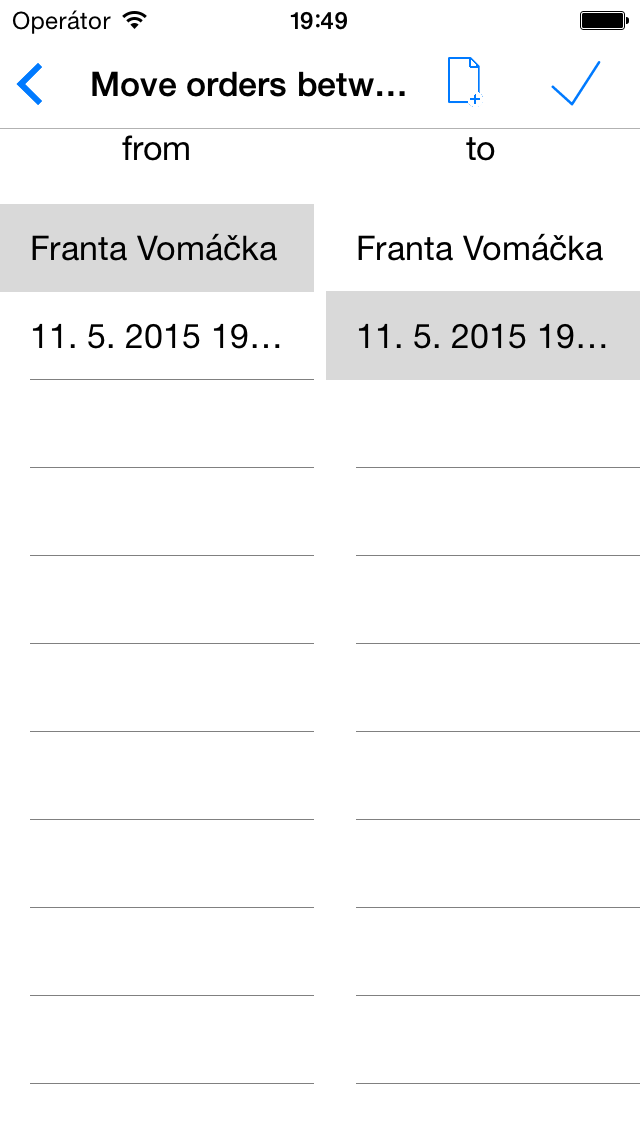
\includegraphics[width=.95\textwidth]{move1.png}
  \captionof{figure}{Přesunout položky\\ mezi účty - výběr účtů}
  \label{fig:moveorderspage1}
\end{minipage}%
\begin{minipage}{.5\textwidth}
  \centering
  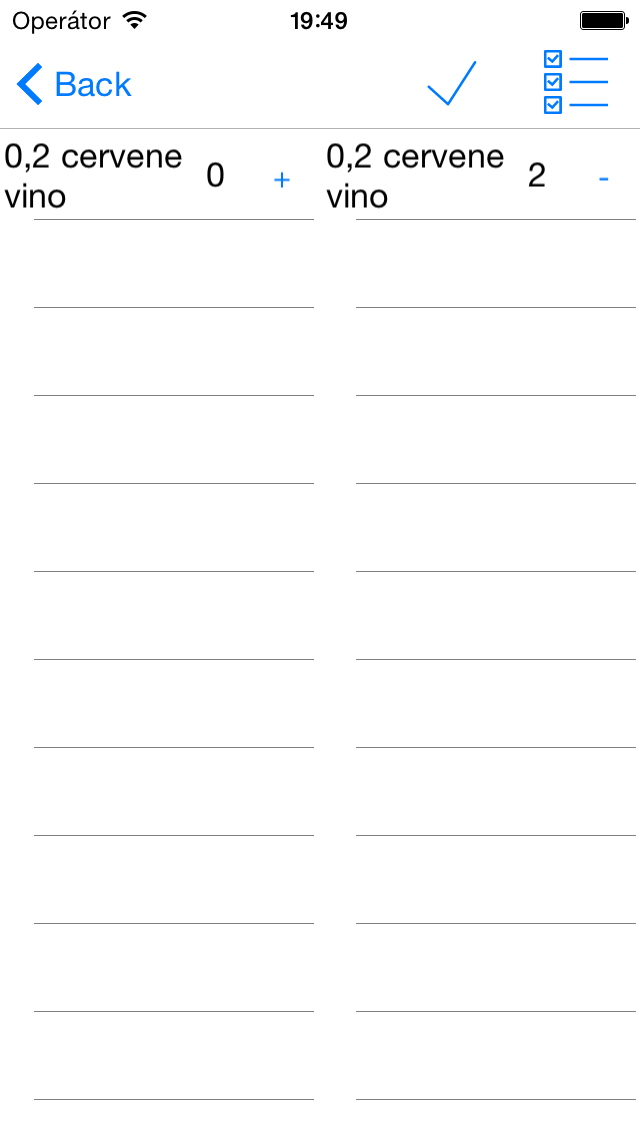
\includegraphics[width=.95\textwidth]{move2.png}
  \captionof{figure}{Přesunout položky\\ mezi účty - výběr položek}
  \label{fig:moveorderspage2}
\end{minipage}
\end{figure}

Druhou funkcí dostupnou z hlavní stránky je vytvoření nového účtu.
Tento dialog je identický pro vytváření účtu z hlavní stránky nebo ze stránky přesouvání položek.
Pokud je dialog prázdný, vypadá jako na obrázku \ref{fig:createaccountpage1}.
V tomto případě nelze vytvořit účet, protože nemá název, ale je možné vytvořit rychloobjednávku.
Tato volba vytvoří účet s časovým údajem jako názvem.
Takovýto účet je určen pro rychlé naplnění a zaplacení.

Pokud specifikujeme název, změní se tlačítko rychloobjednávka na tlačítko vytvořit.
Dále můžeme přidružit k účtu specifický stůl a napsat poznámku.\\

\begin{figure}
\centering
\begin{minipage}{.5\textwidth}
  \centering
  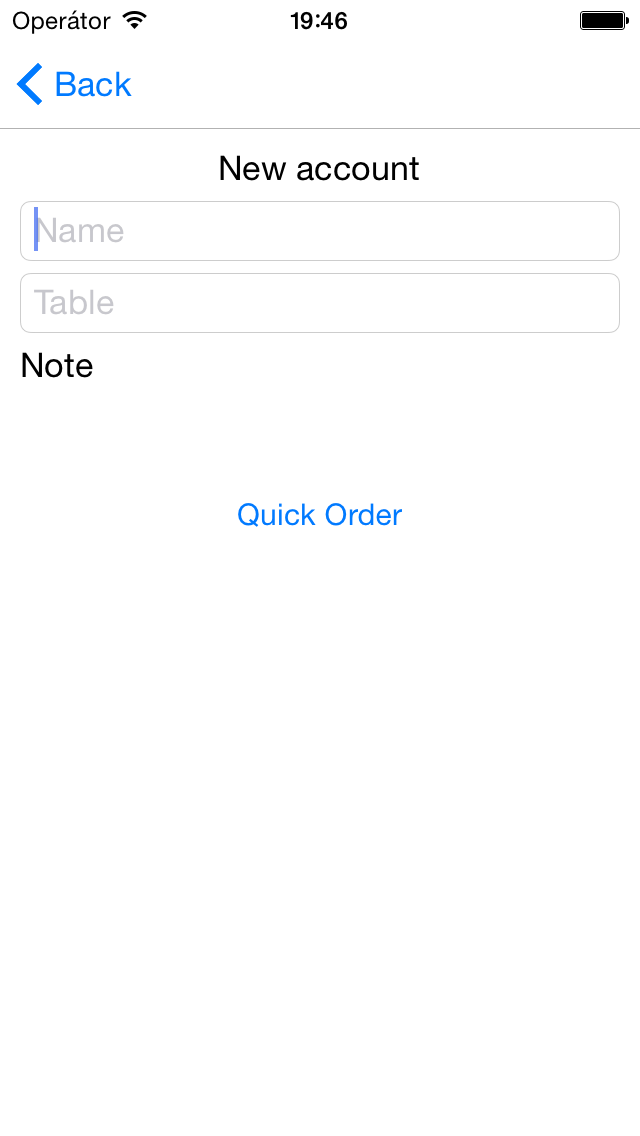
\includegraphics[width=.95\textwidth]{quickorder.png}
  \captionof{figure}{Rychloobjednávka}
  \label{fig:createaccountpage1}
\end{minipage}%
\begin{minipage}{.5\textwidth}
  \centering
  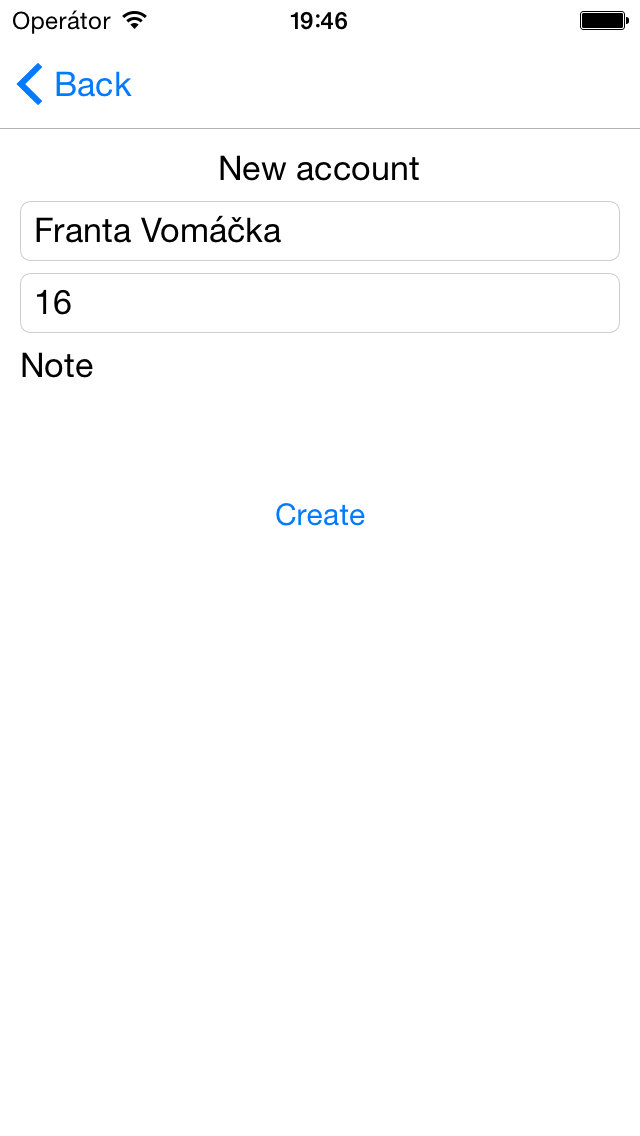
\includegraphics[width=.95\textwidth]{createaccount.png}
  \captionof{figure}{Vytvořit účet}
  \label{fig:createaccountpage2}
\end{minipage}
\end{figure}

Třetí funkcí dostupnou z hlavní stránky je vytvoření objednávky.
Jednotlivé položky dostupné k objednání jsou rozděleny do mřížkového menu (obrázek \ref{fig:createorderpage1}).
Některé položky reprezentují objednatelnou položku, jiné zas podmenu.
V tomto případě se jsou rozděleny do dvou barev: zelené a červené v tomto pořadí.
Zvolené položky se pak plní do postranního panelu viz obrázek \ref{fig:createorderpage2}.
Počet položek jednoho typu lze upravit pomocí příslušného tlačítka mínus.

V liště nástrojů jsou dostupné funkce pro navigaci stromovou strukturou menu.
Ikonky reprezentují zleva do prava přejít o úrověn nahoru, přejít do počáteční úrovně a vytvořit objednávku.\\

\begin{figure}
\centering
\begin{minipage}{.5\textwidth}
  \centering
  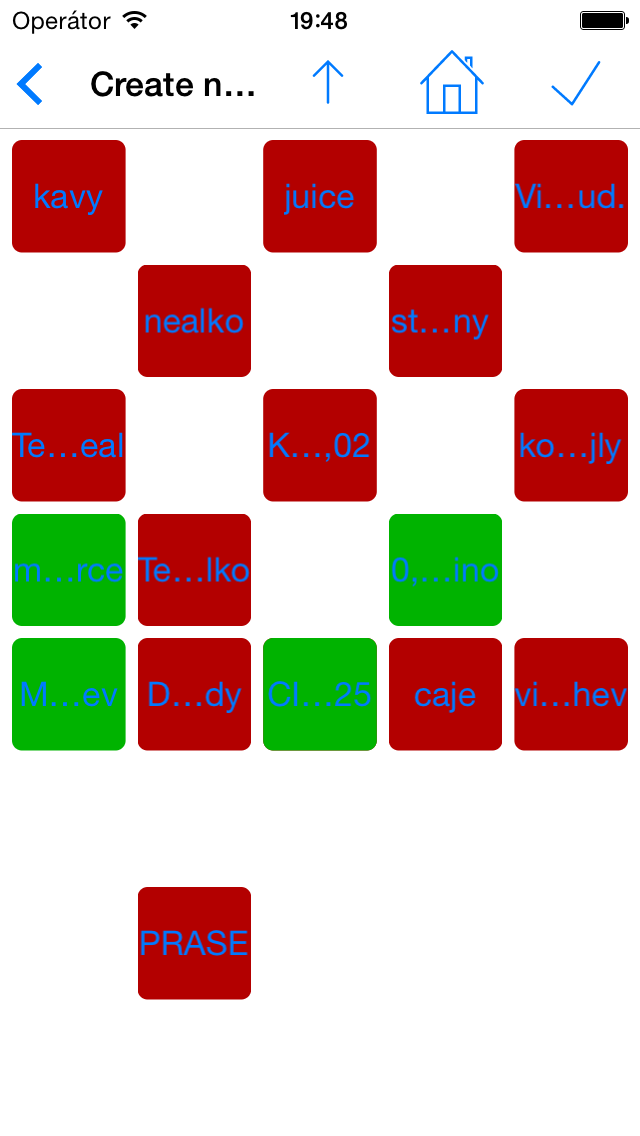
\includegraphics[width=.95\textwidth]{order1.png}
  \captionof{figure}{Vytvořit objednávku}
  \label{fig:createorderpage1}
\end{minipage}%
\begin{minipage}{.5\textwidth}
  \centering
  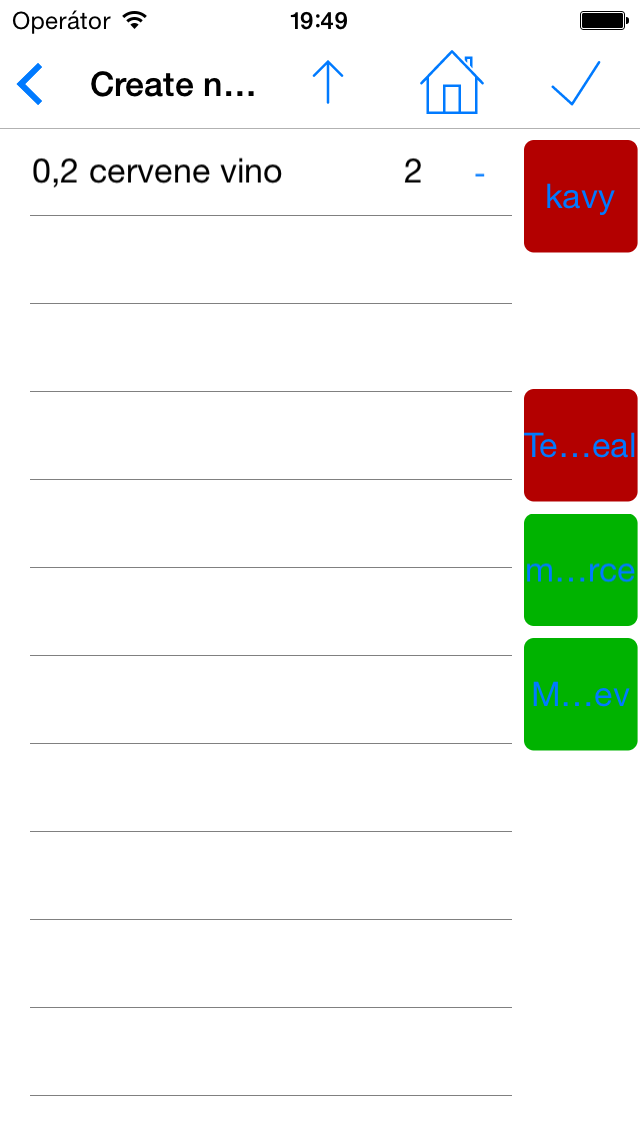
\includegraphics[width=.95\textwidth]{order2.png}
  \captionof{figure}{Vytvořit objednávku - postranní panel}
  \label{fig:createorderpage2}
\end{minipage}
\end{figure}

Poslední funkcí je platba objednávek (obrázek \ref{fig:paypage1}).
Z tohoto dialogu jsou dostupné funkce pro práci s objednávkami.
Jsou to vyčistit výběr, stornovat položky, zaplatit vybrané a zaplatit všechny.
Po vybrání položek se zobrazí druhý dialog, viz obrázek \ref{fig:paypage2}, odkud lze zkontrolovat platbu, zaplatit účet, nebo pouze vytisknout účtenku bez placení.
Poslední tlačítko placení zruší a vrátí uživatele na hlavní obrazovku.

Po zaplacení aplikace automaticky vytisk účtenku.
Pokud v nastavení není nastavena výchozí tiskárna, zobrazí se dialog s výběrem až tří možností.
Aplikace může nabídnout některé z následujících voleb, závisle na tom, které daná platforma podporuje.

\begin{itemize}

\item \textbf{Apple AirPrint}\\
    Tato volba zobrazí systémový dialog pro tisk.
    Účtenku pak lze tisknout s AirPrint kompatibilními WiFi tiskárnami.
\item \textbf{Android Print}\\
    Tato volba zobrazí systémový dialog pro tisk.
    Účtenku pak lze tisknout s podporovanými WiFi tiskárnami nebo uložit jako PDF.
\item \textbf{CashBob Server Print}\\
    Tato volba pošle žádost aplikaci CashBob Server na počítač, která vytiskne účtenku na výchozí tiskárnu počítače.
    Tuto funkci nelze využít s cloudovým serverem, protože k němu není připojená žádná tiskárna.
\item \textbf{Star Portable Printer}\\
    Tato volba umožňuje tisk s mobilní tiskárnou Star Micronics SM-T300.
    Tiskárna musí být připojena k zařízení přes Bluetooth, aby mohla být účtenka vytisknuta.
\end{itemize}

\begin{figure}
\centering
\begin{minipage}{.5\textwidth}
  \centering
  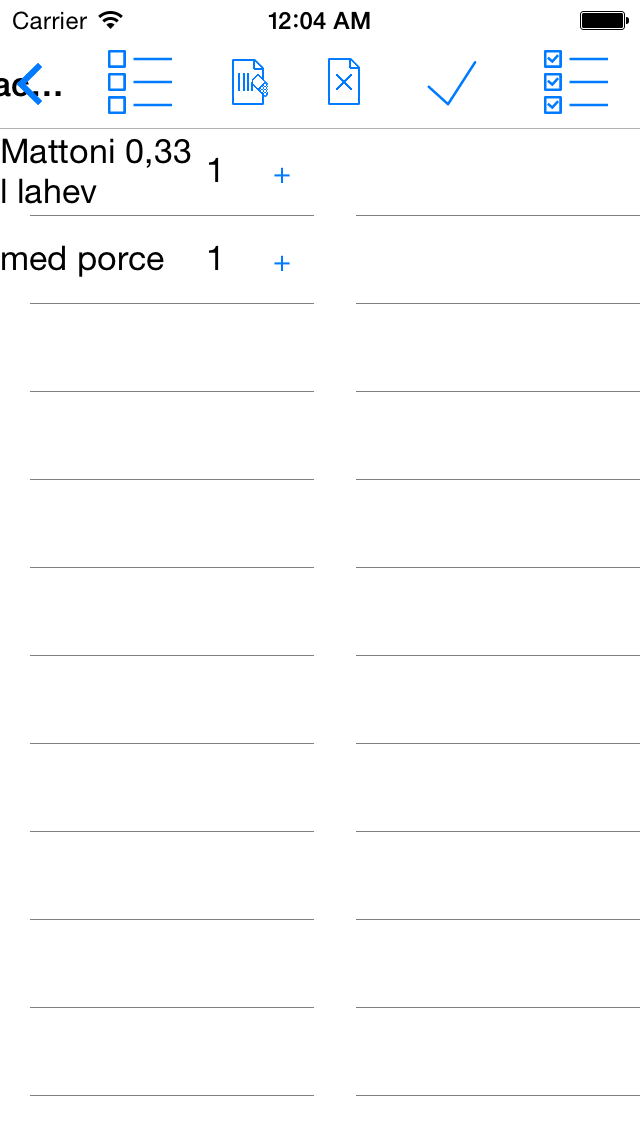
\includegraphics[width=.95\textwidth]{pay1.png}
  \captionof{figure}{Zaplatit - výběr položek}
  \label{fig:paypage1}
\end{minipage}%
\begin{minipage}{.5\textwidth}
  \centering
  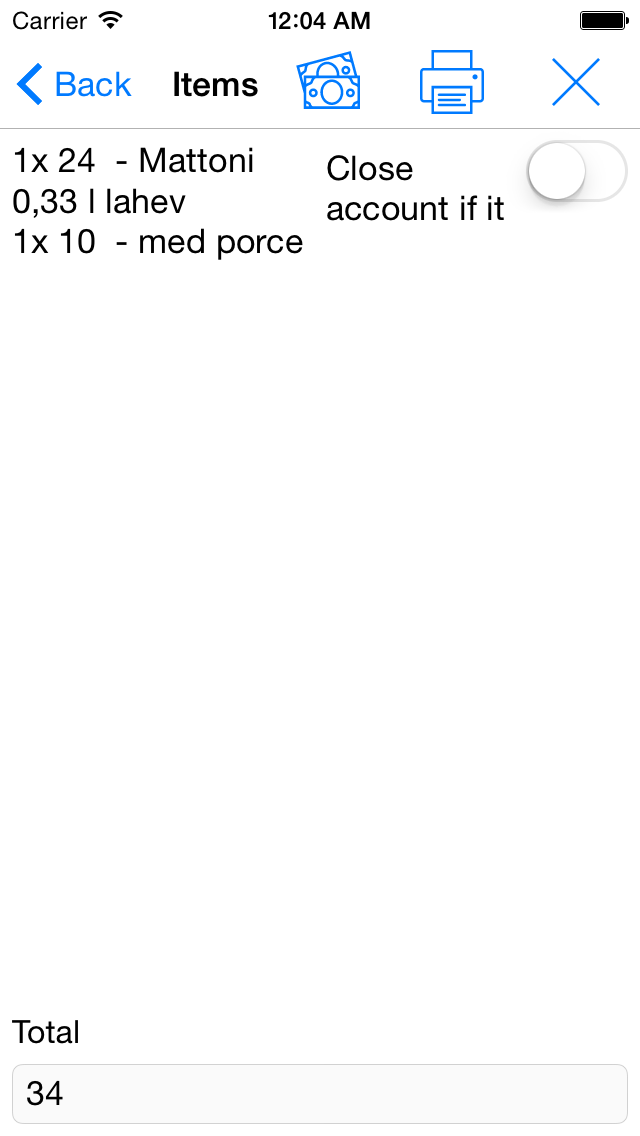
\includegraphics[width=.95\textwidth]{pay2.png}
  \captionof{figure}{Zaplatit - potvrzení}
  \label{fig:paypage2}
\end{minipage}
\end{figure}
\end{document}
